%
% 000-session16.tex
% Presentation Session 16: HTML Forms
%
% Compile to .pdf with LaTeX (pdflatex)
% Requires Beamer package (latex-beamer)
%

\documentclass[xcolor=table]{beamer}
\usetheme{Warsaw}
\beamertemplatenavigationsymbolsempty
\setbeamertemplate{headline}{}
\setbeamerfont{title}{size=\large}
\useoutertheme{infolines}
\usepackage[english]{babel}
\usepackage[utf8]{inputenc}
\usepackage{graphics}
\usepackage{amssymb}
\usepackage{multirow}
\usepackage{xcolor}
\usepackage{framed}
\usepackage{hyperref}
\usepackage{tikz}
\usetikzlibrary{arrows.meta, positioning}

\definecolor{shadecolor}{RGB}{180,180,180}

%%%%%%%%%%%%%%%%%%%%%%%%%%%%%%%%%%%%%%%%%%%%%%%%%%%%%%%%%%%%%%%%
% Python Highlighting
%%%%%%%%%%%%%%%%%%%%%%%%%%%%%%%%%%%%%%%%%%%%%%%%%%%%%%%%%%%%%%%%
\DeclareFixedFont{\ttb}{T1}{txtt}{bx}{n}{10}
\DeclareFixedFont{\ttm}{T1}{txtt}{m}{n}{10}

% Custom colors
\usepackage{color}
\definecolor{deepblue}{rgb}{0,0,0.5}
\definecolor{deepred}{rgb}{0.6,0,0}
\definecolor{deepgreen}{rgb}{0,0.5,0}
\definecolor{grey1}{rgb}{0.5,0.5,0.5}

\usepackage{listings}

% Python style for highlighting
\newcommand\pythonstyle{\lstset{
language=Python,
basicstyle=\ttm\small,
morekeywords={self},
keywordstyle=\ttb\color{deepblue},
emphstyle=\ttb\color{deepred},
stringstyle=\color{deepgreen},
commentstyle=\small\color{grey1}\ttm,
frame=single,
showstringspaces=false
}}

% HTML style for highlighting
\newcommand\htmlstyle{\lstset{
language=HTML,
basicstyle=\ttm\small,
keywordstyle=\ttb\color{deepblue},
stringstyle=\color{deepgreen},
commentstyle=\small\color{grey1}\ttm,
frame=single,
showstringspaces=false
}}

% Python environment
\lstnewenvironment{python}[1][]
{
\pythonstyle
\lstset{#1}
}
{}

% HTML environment
\lstnewenvironment{htmlcode}[1][]
{
\htmlstyle
\lstset{#1}
}
{}

% Python for inline
\newcommand\pythoninline[1]{{\pythonstyle\lstinline!#1!}}

% HTML for inline
\newcommand\htmlinline[1]{{\htmlstyle\lstinline!#1!}}

\newcommand{\asignatura}{Session 16: HTML Forms}
\newcommand{\grado}{Programming in Network Environments}
\newcommand{\curso}{2025-2026}

\title[\asignatura]{\asignatura}
\subtitle{\grado}
\author{URJC}
\institute{GSyC}
\date{Course \curso}

\AtBeginSection[]
{
\begin{frame}<beamer>
\begin{center}
{\LARGE \insertsection}
\end{center}
\end{frame}
}

\begin{document}

\frame{
\maketitle
}

\begin{frame}
\frametitle{Contents}
\tableofcontents
\end{frame}

%%%%%%%%%%%%%%%%%%%%%%%%%%%%%%%%%%%%%%%%%%%%%%%%%%%%%%%%%%%%%%%%
%%%%%%%%%%%%%%%%%%%%%%%%%%%%%%%%%%%%%%%%%%%%%%%%%%%%%%%%%%%%%%%%
% SECTION 1: Introduction to HTML Forms
%%%%%%%%%%%%%%%%%%%%%%%%%%%%%%%%%%%%%%%%%%%%%%%%%%%%%%%%%%%%%%%%
%%%%%%%%%%%%%%%%%%%%%%%%%%%%%%%%%%%%%%%%%%%%%%%%%%%%%%%%%%%%%%%%

\section{Introduction to HTML Forms}

\begin{frame}
\frametitle{Why Do We Need Forms?}

So far, clients can only \textbf{request resources} from the server.

\vspace{0.3cm}

But what if the client needs to \textbf{send data} to the server?

\vspace{0.3cm}

\begin{itemize}
\item A \textbf{search query} (e.g., Google)
\item A \textbf{username and password} (login)
\item \textbf{Text messages} (chat applications)
\item \textbf{Selecting options} (filters, preferences)
\end{itemize}

\vspace{0.4cm}

\begin{center}
$\Rightarrow$ \textbf{HTML Forms} allow clients to \textbf{submit data} to web servers.
\end{center}

\end{frame}

\begin{frame}
\frametitle{How Forms Work}

\begin{center}
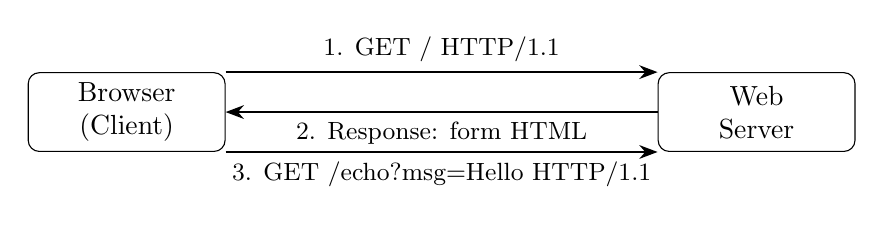
\begin{tikzpicture}[
  box/.style={draw, rounded corners, minimum width=2.5cm, minimum height=1cm, align=center},
  >=Stealth
]
\node[box] (browser) at (0,0) {Browser\\(Client)};
\node[box] (server) at (8,0) {Web\\Server};

\draw[->, thick] (browser.north east) -- node[above, font=\small] {1. GET / HTTP/1.1} (server.north west);
\draw[<-, thick] (browser.east) -- node[below, font=\small] {2. Response: form HTML} (server.west);
\draw[->, thick] (browser.south east) -- node[below, font=\small] {3. GET /echo?msg=Hello HTTP/1.1} (server.south west);
\end{tikzpicture}
\end{center}

\vspace{0.3cm}

\begin{enumerate}
\item Client requests the \textbf{main page}
\item Server responds with an HTML page containing a \textbf{form}
\item User fills the form and clicks \textbf{Submit} $\rightarrow$ browser sends a \textbf{new GET request} with the data in the \textbf{URL}
\end{enumerate}

\end{frame}

%%%%%%%%%%%%%%%%%%%%%%%%%%%%%%%%%%%%%%%%%%%%%%%%%%%%%%%%%%%%%%%%
%%%%%%%%%%%%%%%%%%%%%%%%%%%%%%%%%%%%%%%%%%%%%%%%%%%%%%%%%%%%%%%%
% SECTION 2: Our First Form
%%%%%%%%%%%%%%%%%%%%%%%%%%%%%%%%%%%%%%%%%%%%%%%%%%%%%%%%%%%%%%%%
%%%%%%%%%%%%%%%%%%%%%%%%%%%%%%%%%%%%%%%%%%%%%%%%%%%%%%%%%%%%%%%%

\section{Our First Form}

\begin{frame}[fragile]
\frametitle{A Simple Form: HTML Code}

\begin{htmlcode}
<!DOCTYPE html>
<html lang="en">
  <head>
    <meta charset="utf-8">
    <title>FORM 1</title>
  </head>
  <body>
    <form action="echo" method="get">
      Message to send to the server: <br>
      <input type="text" name="msg">
      <input type="submit" value="SEND">
    </form>
  </body>
</html>
\end{htmlcode}

\vspace{0.1cm}

Save as \texttt{html/form-1.html} and open it in the browser.

\end{frame}

\begin{frame}
\frametitle{Understanding the Form Elements}

\begingroup\small
\begin{center}
\begin{tabular}{|l|p{6cm}|}
\hline
\textbf{HTML Element} & \textbf{Purpose} \\
\hline
\texttt{<form>} & Container for all input elements \\
\hline
\texttt{action="echo"} & The \textbf{resource} to request when submitting (the server endpoint) \\
\hline
\texttt{method="get"} & Use HTTP \textbf{GET} method (data goes in the URL) \\
\hline
\texttt{<input type="text">} & A \textbf{text box} for user input \\
\hline
\texttt{name="msg"} & The \textbf{parameter name} sent to the server \\
\hline
\texttt{<input type="submit">} & A \textbf{button} that submits the form \\
\hline
\end{tabular}
\end{center}
\endgroup

\vspace{0.3cm}

When the user types ``Testing...'' and clicks SEND, the browser sends:

\vspace{0.1cm}

\begin{center}
\texttt{GET /echo?msg=Testing... HTTP/1.1}
\end{center}

\end{frame}

\begin{frame}
\frametitle{The Query String}

The data from the form is appended to the URL as a \textbf{query string}:

\vspace{0.2cm}

\begin{center}
\texttt{/echo\textbf{?msg=Testing...}}
\end{center}

\vspace{0.2cm}

\begin{itemize}
\item \texttt{?} separates the \textbf{path} from the \textbf{parameters}
\item \texttt{msg=Testing...} is a \textbf{key=value} pair
\item The \textbf{key} comes from the \texttt{name} attribute of the input
\item The \textbf{value} is what the user typed
\end{itemize}

\vspace{0.3cm}

With \textbf{multiple parameters}, they are separated by \texttt{\&}:

\vspace{0.1cm}

\begin{center}
\texttt{/myserver?msg=Hello\&base=A\&chk=on}
\end{center}

\end{frame}

%%%%%%%%%%%%%%%%%%%%%%%%%%%%%%%%%%%%%%%%%%%%%%%%%%%%%%%%%%%%%%%%
%%%%%%%%%%%%%%%%%%%%%%%%%%%%%%%%%%%%%%%%%%%%%%%%%%%%%%%%%%%%%%%%
% SECTION 3: Happy Web Server with Forms
%%%%%%%%%%%%%%%%%%%%%%%%%%%%%%%%%%%%%%%%%%%%%%%%%%%%%%%%%%%%%%%%
%%%%%%%%%%%%%%%%%%%%%%%%%%%%%%%%%%%%%%%%%%%%%%%%%%%%%%%%%%%%%%%%

\section{Happy Web Server with Forms}

\begin{frame}[fragile]
\frametitle{Testing Forms: The Happy Server}

A server that \textbf{always returns the form}, regardless of the request:

\vspace{0.1cm}

\begin{python}
class TestHandler(
        http.server.BaseHTTPRequestHandler):

    def do_GET(self):
        termcolor.cprint(self.requestline, 'green')

        contents = Path(
            'html/form-1.html').read_text()

        self.send_response(200)
        self.send_header('Content-Type','text/html')
        self.send_header('Content-Length',
                         len(contents.encode()))
        self.end_headers()
        self.wfile.write(contents.encode())
\end{python}

\end{frame}

\begin{frame}
\frametitle{What Happens in the Console?}

Run the server, connect from the browser, type a message and click SEND.

\vspace{0.3cm}

The server console shows \textbf{two requests}:

\vspace{0.2cm}

\begin{enumerate}
\item \texttt{GET / HTTP/1.1} -- requesting the \textbf{main page}
\item \texttt{GET /echo?msg=abcdefg HTTP/1.1} -- \textbf{submitting} the form data
\end{enumerate}

\vspace{0.3cm}

The second request contains:
\begin{itemize}
\item \textbf{Path}: \texttt{/echo} (the \texttt{action} attribute)
\item \textbf{Parameter}: \texttt{msg=abcdefg} (the text input value)
\end{itemize}

\vspace{0.2cm}

The server responds with the form again (it is a \textbf{happy server} -- always the same response).

\end{frame}

%%%%%%%%%%%%%%%%%%%%%%%%%%%%%%%%%%%%%%%%%%%%%%%%%%%%%%%%%%%%%%%%
%%%%%%%%%%%%%%%%%%%%%%%%%%%%%%%%%%%%%%%%%%%%%%%%%%%%%%%%%%%%%%%%
% SECTION 4: Types of Input Elements
%%%%%%%%%%%%%%%%%%%%%%%%%%%%%%%%%%%%%%%%%%%%%%%%%%%%%%%%%%%%%%%%
%%%%%%%%%%%%%%%%%%%%%%%%%%%%%%%%%%%%%%%%%%%%%%%%%%%%%%%%%%%%%%%%

\section{Types of Input Elements}

\begin{frame}[fragile]
\frametitle{Beyond Text: Other Input Types}

HTML provides many \textbf{input types} for forms:

\vspace{0.2cm}

\begingroup\small
\begin{center}
\begin{tabular}{|l|l|l|}
\hline
\textbf{Type} & \textbf{HTML} & \textbf{Description} \\
\hline
Text box & \texttt{<input type="text">} & Free text input \\
\hline
Checkbox & \texttt{<input type="checkbox">} & On/off toggle \\
\hline
Radio & \texttt{<input type="radio">} & Select one from a group \\
\hline
Dropdown & \texttt{<select>...<option>} & Choose from a list \\
\hline
Submit & \texttt{<input type="submit">} & Send the form \\
\hline
\end{tabular}
\end{center}
\endgroup

\end{frame}

\begin{frame}[fragile]
\frametitle{Form with Multiple Input Types}

\begin{htmlcode}[basicstyle=\ttm\scriptsize]
<form action="myserver" method="get">
  Text input
  <input type="text" name="msg">
  <br><br>
  Check button:
  <input type="checkbox" name="chk">
  <br><br>
  Radio buttons:
  <input type="radio" name="base" value="A"
         checked> A
  <input type="radio" name="base" value="C"> C
  <input type="radio" name="base" value="T"> T
  <input type="radio" name="base" value="G"> G
  <br><br>
  Choose operation:
  <select name="operation">
    <option value="count">Count</option>
    <option value="perc">Percentage</option>
  </select>
  <br>
  <input type="submit"/>
</form>
\end{htmlcode}

\end{frame}

\begin{frame}
\frametitle{Generated Request with Multiple Inputs}

When the user fills the form and clicks submit, \textbf{all inputs} are sent as parameters:

\vspace{0.3cm}

\begin{center}
\texttt{GET /myserver?msg=Hello\&chk=on\&base=A\&operation=count HTTP/1.1}
\end{center}

\vspace{0.3cm}

\begin{itemize}
\item \textbf{Text}: \texttt{msg=Hello}
\item \textbf{Checkbox}: \texttt{chk=on} (only sent if \textbf{checked})
\item \textbf{Radio}: \texttt{base=A} (the \texttt{value} of the selected option)
\item \textbf{Dropdown}: \texttt{operation=count} (the selected \texttt{<option>})
\end{itemize}

\vspace{0.3cm}

Each input's \texttt{name} attribute becomes the \textbf{key} in the query string.

\end{frame}

%%%%%%%%%%%%%%%%%%%%%%%%%%%%%%%%%%%%%%%%%%%%%%%%%%%%%%%%%%%%%%%%
%%%%%%%%%%%%%%%%%%%%%%%%%%%%%%%%%%%%%%%%%%%%%%%%%%%%%%%%%%%%%%%%
% SECTION 5: Parsing Form Data in the Server
%%%%%%%%%%%%%%%%%%%%%%%%%%%%%%%%%%%%%%%%%%%%%%%%%%%%%%%%%%%%%%%%
%%%%%%%%%%%%%%%%%%%%%%%%%%%%%%%%%%%%%%%%%%%%%%%%%%%%%%%%%%%%%%%%

\section{Parsing Form Data in the Server}

\begin{frame}[fragile]
\frametitle{Extracting Path and Arguments}

Use \pythoninline{urllib.parse} to separate the \textbf{path} from the \textbf{parameters}:

\vspace{0.1cm}

\begin{python}
from urllib.parse import parse_qs, urlparse

# Inside do_GET():
url_path = urlparse(self.path)
path = url_path.path       # "/echo"
arguments = parse_qs(url_path.query)
# {"msg": ["Hello"]}
\end{python}

\vspace{0.2cm}

\textbf{Without} \pythoninline{urlparse}, \pythoninline{self.path} would be:

\vspace{0.1cm}

\begin{center}
\texttt{/echo?msg=Hello} $\leftarrow$ path and params mixed together
\end{center}

\vspace{0.2cm}

\textbf{With} \pythoninline{urlparse}, we get them \textbf{separated}:

\begin{itemize}
\item \pythoninline{path} $\rightarrow$ \texttt{"/echo"}
\item \pythoninline{arguments} $\rightarrow$ \pythoninline{\{"msg": ["Hello"]\}}
\end{itemize}

\end{frame}

\begin{frame}[fragile]
\frametitle{Dynamic HTML with Jinja2 Templates}

Use \pythoninline{jinja2} to generate \textbf{dynamic HTML} with data from the form:

\vspace{0.1cm}

\begin{python}
import jinja2 as j
from pathlib import Path

def read_html_file(filename):
    contents = Path(
        "html/" + filename).read_text()
    contents = j.Template(contents)
    return contents

# Render with data from the form
contents = read_html_file("echo.html").render(
    context={"todisplay": text})
\end{python}

\vspace{0.2cm}

In the HTML file, use \texttt{\{\{context.todisplay\}\}} where you want the text:

\vspace{0.1cm}

\begin{center}
\texttt{<p>\{\{context.todisplay\}\}</p>}
\end{center}

\end{frame}

%%%%%%%%%%%%%%%%%%%%%%%%%%%%%%%%%%%%%%%%%%%%%%%%%%%%%%%%%%%%%%%%
%%%%%%%%%%%%%%%%%%%%%%%%%%%%%%%%%%%%%%%%%%%%%%%%%%%%%%%%%%%%%%%%
% SECTION 6: Exercises
%%%%%%%%%%%%%%%%%%%%%%%%%%%%%%%%%%%%%%%%%%%%%%%%%%%%%%%%%%%%%%%%
%%%%%%%%%%%%%%%%%%%%%%%%%%%%%%%%%%%%%%%%%%%%%%%%%%%%%%%%%%%%%%%%

\section{Exercises}

\begin{frame}
\frametitle{Exercise 1: Echo Server}

\textbf{Files}: \texttt{S16/echo-server-e1.py}, \texttt{S16/html/form-e1.html}, \texttt{S16/html/error.html}

\vspace{0.2cm}

\textbf{Description}:
\begin{itemize}
\item Request \texttt{/} $\rightarrow$ return a form with a \textbf{text input} and \textbf{submit button}
\item Form submits to \texttt{/echo} $\rightarrow$ server responds with an HTML page showing the \textbf{user's message}
\item Include a \textbf{link} at the bottom to return to the main form
\item Any other resource $\rightarrow$ return an \textbf{error page} (also with a link back)
\end{itemize}

\vspace{0.2cm}

\textbf{Hints}:
\begin{itemize}
\item Use \pythoninline{urlparse} to separate path from arguments
\item Use \pythoninline{jinja2} to render the echo response dynamically
\item Check \pythoninline{path == "/echo"} to know when form data arrives
\end{itemize}

\end{frame}

\begin{frame}
\frametitle{Exercise 2: Echo Server with Check Button}

\textbf{Files}: \texttt{S16/echo-server-e2.py}, \texttt{S16/html/form-e2.html}

\vspace{0.3cm}

\textbf{Description}:
\begin{itemize}
\item Modify Exercise 1 to add a \textbf{checkbox} to the form
\item When the checkbox is \textbf{checked}, the echo message is shown in \textbf{CAPITAL LETTERS}
\item When it is \textbf{unchecked}, the echo is shown normally
\end{itemize}

\vspace{0.3cm}

\textbf{Hints}:
\begin{itemize}
\item Add \texttt{<input type="checkbox" name="chk">} to the form
\item In the server, check if \texttt{"chk"} is in the arguments
\item If present, convert the message with \pythoninline{.upper()}
\end{itemize}

\end{frame}

\begin{frame}
\frametitle{Deliverables}

\textbf{S16 folder should contain}:

\vspace{0.2cm}

\begingroup\small
\begin{itemize}
\item \texttt{form-server1.py} -- Happy server (from the examples)
\item \texttt{html/form-1.html} -- Simple form
\item \texttt{html/form-2.html} -- Form with multiple inputs
\item \texttt{echo-server-e1.py} -- Echo server (Exercise 1)
\item \texttt{html/form-e1.html} -- Echo form
\item \texttt{html/error.html} -- Error page
\item \texttt{echo-server-e2.py} -- Echo server with checkbox (Exercise 2)
\item \texttt{html/form-e2.html} -- Echo form with checkbox
\end{itemize}
\endgroup

\vspace{0.3cm}

\textbf{Remember}: Push everything to your remote Gitlab repo!

\end{frame}

%%%%%%%%%%%%%%%%%%%%%%%%%%%%%%%%%%%%%%%%%%%%%%%%%%%%%%%%%%%%%%%%
%%%%%%%%%%%%%%%%%%%%%%%%%%%%%%%%%%%%%%%%%%%%%%%%%%%%%%%%%%%%%%%%
% SECTION 7: End
%%%%%%%%%%%%%%%%%%%%%%%%%%%%%%%%%%%%%%%%%%%%%%%%%%%%%%%%%%%%%%%%
%%%%%%%%%%%%%%%%%%%%%%%%%%%%%%%%%%%%%%%%%%%%%%%%%%%%%%%%%%%%%%%%

\begin{frame}
\begin{center}
\Huge{Questions?}

\vspace{1cm}

\Large{Time to code!}
\end{center}
\end{frame}

\end{document}
